\begin{pastexam}[label={px:gw3-098-ds-02}]{關務三等資訊處理 98 年 第二題}
（申論；20 分）

圖形（graph）$G$ 有 12 個節點（node），分別用數字 0, 1, 2, 3, 6, 7, 8, 9, 12, 13, 14, 15 標記。標記為 $a$, $b$ 的
兩個節點間有邊線（edge），若且唯若 $a = a_1a_2a_3a_4$, $b = b_1b_2b_3b_4$ 的四位元二進位表示法恰有一個位元不相同。
例如 1 = 0001, 3 = 0011, 9 = 1001, 則標記為 3 的節點與標記為 1 的節點間有邊線，與標記為 9 的節點間沒有邊線。
\begin{enumerate}[leftmargin=2.6em, labelsep=0.4em]
\item[㈠] 請分別用鄰接矩陣（adjacency matrix）與鄰接串列（adjacency list）的方式表示圖形 $G$。（10 分）
\item[㈡] 請在標記小的節點先搜尋的規則下，產生以節點 0 為起始節點的廣度優先搜尋擴張樹（breadth-first search
spanning tree）與深度優先搜尋擴張樹（depth-first search spanning tree）。（10 分）
\end{enumerate}
\end{pastexam}

\begin{pastsoln}
\textbf{先找邊}。 和 $a$ 恰差一個位元的數是 $a \oplus 1$、$a \oplus 2$、$a \oplus 4$、$a \oplus 8$（$\oplus$ 是逐位元
互斥或），其中出現在節點集合裡的才是鄰居。 節點集合少了 $4, 5, 10, 11$（$0100$、$0101$、$1010$、$1011$）。
\begin{center}
\small
\begin{tabular}{cccl}
\toprule
節點 & 二進位 & 翻一個位元得到的四個數 & 鄰居（在集合裡的） \\
\midrule
0 & 0000 & 1, 2, 4, 8 & 1, 2, 8 \\
1 & 0001 & 0, 3, 5, 9 & 0, 3, 9 \\
2 & 0010 & 3, 0, 6, 10 & 0, 3, 6 \\
3 & 0011 & 2, 1, 7, 11 & 1, 2, 7 \\
6 & 0110 & 7, 4, 2, 14 & 2, 7, 14 \\
7 & 0111 & 6, 5, 3, 15 & 3, 6, 15 \\
8 & 1000 & 9, 10, 12, 0 & 0, 9, 12 \\
9 & 1001 & 8, 11, 13, 1 & 1, 8, 13 \\
12 & 1100 & 13, 14, 8, 4 & 8, 13, 14 \\
13 & 1101 & 12, 15, 9, 5 & 9, 12, 15 \\
14 & 1110 & 15, 12, 6, 10 & 6, 12, 15 \\
15 & 1111 & 14, 13, 7, 11 & 7, 13, 14 \\
\bottomrule
\end{tabular}
\end{center}
每個節點度數都是 $3$，共 $12 \times 3 / 2 = 18$ 條邊。

\textbf{㈠ 鄰接矩陣}（資結書第~21.2~節）：$12 \times 12$，列、行依標記由小到大排，$M[u][v] = 1$ 表示有邊。
無向圖，矩陣對稱，對角線為 $0$。
\begin{center}
\small
\setlength{\tabcolsep}{4pt}
\begin{tabular}{c|cccccccccccc}
 & 0 & 1 & 2 & 3 & 6 & 7 & 8 & 9 & 12 & 13 & 14 & 15 \\
\hline
0 & 0 & 1 & 1 & 0 & 0 & 0 & 1 & 0 & 0 & 0 & 0 & 0 \\
1 & 1 & 0 & 0 & 1 & 0 & 0 & 0 & 1 & 0 & 0 & 0 & 0 \\
2 & 1 & 0 & 0 & 1 & 1 & 0 & 0 & 0 & 0 & 0 & 0 & 0 \\
3 & 0 & 1 & 1 & 0 & 0 & 1 & 0 & 0 & 0 & 0 & 0 & 0 \\
6 & 0 & 0 & 1 & 0 & 0 & 1 & 0 & 0 & 0 & 0 & 1 & 0 \\
7 & 0 & 0 & 0 & 1 & 1 & 0 & 0 & 0 & 0 & 0 & 0 & 1 \\
8 & 1 & 0 & 0 & 0 & 0 & 0 & 0 & 1 & 1 & 0 & 0 & 0 \\
9 & 0 & 1 & 0 & 0 & 0 & 0 & 1 & 0 & 0 & 1 & 0 & 0 \\
12 & 0 & 0 & 0 & 0 & 0 & 0 & 1 & 0 & 0 & 1 & 1 & 0 \\
13 & 0 & 0 & 0 & 0 & 0 & 0 & 0 & 1 & 1 & 0 & 0 & 1 \\
14 & 0 & 0 & 0 & 0 & 1 & 0 & 0 & 0 & 1 & 0 & 0 & 1 \\
15 & 0 & 0 & 0 & 0 & 0 & 1 & 0 & 0 & 0 & 1 & 1 & 0 \\
\end{tabular}
\end{center}
\textbf{鄰接串列}：每個節點一個串列頭，串列裡依標記由小到大放鄰居（每條無向邊在兩端各出現一次，共 $36$ 個串列節點）：
\begin{center}
\small
\begin{tabular}{l@{\qquad}l}
$0 \to 1 \to 2 \to 8$ & $7 \to 3 \to 6 \to 15$ \\
$1 \to 0 \to 3 \to 9$ & $8 \to 0 \to 9 \to 12$ \\
$2 \to 0 \to 3 \to 6$ & $9 \to 1 \to 8 \to 13$ \\
$3 \to 1 \to 2 \to 7$ & $12 \to 8 \to 13 \to 14$ \\
$6 \to 2 \to 7 \to 14$ & $13 \to 9 \to 12 \to 15$ \\
 & $14 \to 6 \to 12 \to 15$ \\
 & $15 \to 7 \to 13 \to 14$ \\
\end{tabular}
\end{center}
（每個串列最後接 \NIL。）

\textbf{㈡ BFS 擴張樹}（資結書第~21.3~節）：從 $0$ 開始，取出佇列前端的節點，依標記由小到大看鄰居，沒拜訪過的
就加入樹（父節點是目前節點）並放進佇列。
\begin{center}
\small
\begin{tabular}{clll}
\toprule
取出 & 鄰居 & 新加入（父） & 佇列（處理後） \\
\midrule
0 & 1, 2, 8 & 1, 2, 8（父 0） & 1, 2, 8 \\
1 & 0, 3, 9 & 3, 9（父 1） & 2, 8, 3, 9 \\
2 & 0, 3, 6 & 6（父 2） & 8, 3, 9, 6 \\
8 & 0, 9, 12 & 12（父 8） & 3, 9, 6, 12 \\
3 & 1, 2, 7 & 7（父 3） & 9, 6, 12, 7 \\
9 & 1, 8, 13 & 13（父 9） & 6, 12, 7, 13 \\
6 & 2, 7, 14 & 14（父 6） & 12, 7, 13, 14 \\
12 & 8, 13, 14 & 無 & 7, 13, 14 \\
7 & 3, 6, 15 & 15（父 7） & 13, 14, 15 \\
13, 14, 15 & & 無 & 空 \\
\bottomrule
\end{tabular}
\end{center}
拜訪順序 0, 1, 2, 8, 3, 9, 6, 12, 7, 13, 14, 15。 樹邊：(0,\,1)、(0,\,2)、(0,\,8)、(1,\,3)、(1,\,9)、(2,\,6)、
(8,\,12)、(3,\,7)、(9,\,13)、(6,\,14)、(7,\,15)，共 $11$ 條。
\begin{center}
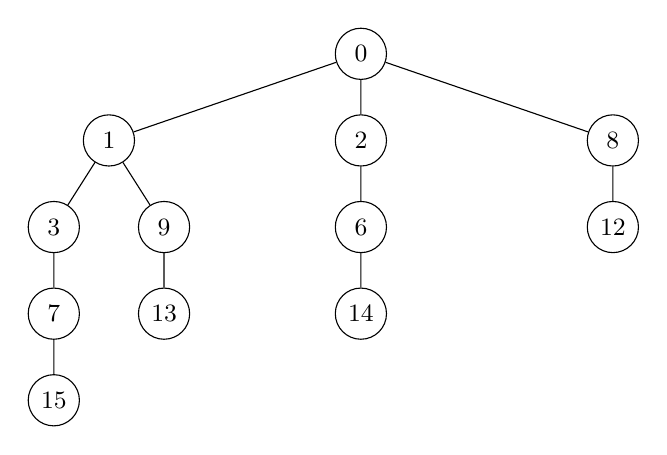
\begin{tikzpicture}[n/.style={circle,draw,inner sep=0pt,minimum size=6.5mm,font=\small},
  level distance=11mm, level 1/.style={sibling distance=32mm}, level 2/.style={sibling distance=14mm}]
\node[n] {0}
  child {node[n] {1} child {node[n] {3} child {node[n] {7} child {node[n] {15}}}} child {node[n] {9} child {node[n] {13}}}}
  child {node[n] {2} child {node[n] {6} child {node[n] {14}}}}
  child {node[n] {8} child {node[n] {12}}};
\end{tikzpicture}
\end{center}
每個節點在樹上的深度就是它和 $0$ 差幾個位元（$15 = 1111$ 最深，深度 $4$），因為沿著樹邊每走一步翻一個位元，
而且 BFS 樹給出最短距離。

\textbf{DFS 擴張樹}（資結書第~21.4~節）：從 $0$ 開始，每到一個節點，就找標記最小、還沒拜訪的鄰居往下走；
沒有就退回上一個節點。
\begin{itemize}
\item $0 \to 1$（$0$ 最小的鄰居）$\to 3$（$1$ 的鄰居 $0$ 已拜訪）$\to 2$（$3$ 的鄰居 $1$ 已拜訪）$\to 6$（$2$ 的鄰居 $0, 3$ 已拜訪）
\item $6 \to 7$（$2$ 已拜訪）$\to 15$（$3, 6$ 已拜訪）$\to 13$（$7$ 已拜訪）$\to 9$ $\to 8$（$1$ 已拜訪）$\to 12$（$0, 9$ 已拜訪）
$\to 14$（$8, 13$ 已拜訪）。
\item $14$ 的鄰居 $6, 12, 15$ 都已拜訪，一路退回 $0$，結束。
\end{itemize}
拜訪順序 0, 1, 3, 2, 6, 7, 15, 13, 9, 8, 12, 14。 這次 DFS 沒有分岔，樹是一條路徑（經過全部 $12$ 個節點）：
\begin{center}
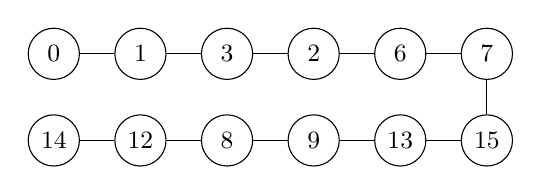
\begin{tikzpicture}[n/.style={circle,draw,inner sep=0pt,minimum size=6.5mm,font=\small}, x=1.1cm]
\foreach \v [count=\i] in {0,1,3,2,6,7}{ \node[n] (a\i) at (\i,0) {\v}; }
\foreach \v [count=\i] in {14,12,8,9,13,15}{ \node[n] (b\i) at (\i,-1.1) {\v}; }
\foreach \i [evaluate=\i as \j using int(\i+1)] in {1,...,5}{ \draw (a\i) -- (a\j); \draw (b\i) -- (b\j); }
\draw (a6) -- (b6);
\end{tikzpicture}
\end{center}
（從左上的 $0$ 出發，沿著路徑走到左下的 $14$。）
\end{pastsoln}
